%%%%%%%%%%%%%%%%%%%%%%%%%%%%%%%%%%%%%%%%%%%%%%%
%
%   Families of Traffic Forecasting Problems
%
%%%%%%%%%%%%%%%%%%%%%%%%%%%%%%%%%%%%%%%%%%%%%%%

%\usepackage{cite}
%\usepackage{multirow}
%\usepackage{rotating} 
%\usepackage[table,xcdraw]{xcolor}
%\usepackage{float}
%\usepackage[utf8]{inputenc}
%\usepackage{amsmath,amssymb,amsfonts}
%\usepackage{algorithmic}
%\usepackage{graphicx}
%\usepackage{textcomp}
%\usepackage{rotating}
%\usepackage{verbatim}


\section{Experimental Results}
\label{sec:4_5_Expsetup}

The objective of the experiments conducted in this study was to evaluate the efficacy of multiclass oversampling techniques in enhancing the performance of the proposed method in imbalanced drifted multiclass classification streams. Our primary goal was to develop a novel approach that combines Dynamic Ensemble Selection (DES) to improve classification accuracy and robustness in such streams. These experiments yielded valuable insights that could further refine the performance of the proposed approach and its ability to effectively handle imbalanced data streams. These findings provide a better understanding of the capabilities of the proposed approach and offer insights into an optimal strategy for tackling minority class issues and concept drift in imbalanced data streams. This study contributes to the advancement of stream mining techniques for generating more accurate and robust classification models in dynamic data stream environments. By addressing the challenges posed by minority classes and concept drift, this study offers valuable insights for improving the performance of the proposed approach and enhancing the overall efficiency of stream mining. The two main questions to be answered are:

\begin{itemize}
  \setlength{\itemindent}{-.5in}
  
      \item $\pmb{Q_1}$: What is the impact of reduced and consistent data on the performance of ensemble learning?
      \item  $\pmb{Q_2}$: Is it possible with the search capability of swarm intelligence to enhance the combination of classifiers? 
  \end{itemize}

\subsection{Experimental setup}
The evaluation of the proposed method incorporated the utilization of various metrics such as recall, precision, specificity, f1 score, balanced accuracy score (BAC), and geometric mean score (G-mean) \cite{bu2016pdf}. The experimental protocol utilized for evaluation was the test-then-train approach \cite{venkatasubramanianinformation}, where the classification classifier was trained on a specific data chunk and subsequently evaluated on the subsequent one. The chunk size was standardized for all utilized data streams to 2,000 instances. We employed four classification classifiers as base estimators: K-Nearest Neighbor (KNN), Support Vector Machine (SVM), Gaussian Naive Bayes (GNB), and Hoeffding Tree (HT), as implemented in scikit-learn \cite{frias2014online}. A pool of classifiers was constructed with a maximum size of L = 8, where the DES selected the best classifier for each chunk. If the pool surpassed the set threshold (L), the classifier with the lowest performance was eliminated. The experiments were conducted using Python programming language, and the source code was publicly available on GitHub\footnote{\url{https://github.com/Amadkour/dynamic__classification_ensembles_for_handling_imbalanced_multi-class_drifted_data_streams.git}} . We conducted a comparison between multiclass oversampling techniques (MLSMOTE and MLSOL) and our proposed approach to demonstrate the effectiveness of our contribution. Additionally, we conducted these experiments using two different concept drift detectors, ADWIN \cite{storkey2008training} and DDM \cite{losing2016knn}, to demonstrate the adaptability and robustness of our proposed approach across varying drift detectors.

\subsection{Data Streams}
In this study, the proposed approach was assessed using various datasets including benchmark datasets, a real application stream dataset, and synthetic data streams. The Stream-learn Python library was used to conduct the evaluations \cite{dries2009adaptive}. Table \ref{tab:4_first_proposal_result_table_1} illustrates the benchmark dataset employed in this study, which consists of the Covertype dataset containing 40 features, seven classes, and 581,010 instances. For real application stream evaluation, the Sensor stream dataset was used, which consisted of five features, 58 classes, and 392,600 instances. This represents a real-world application scenario and provides valuable insights into the performance of the proposed approach in practical settings. Synthetic datasets were generated using Scikit-learn Python library to evaluate the performance of the proposed approach. The synthetic dataset was designed to simulate data streams and comprised 10 features and four classes divided into 200 chunks of 2,000 instances each. The performance of the proposed approach was systematically evaluated using these datasets and a stream-learn library. These evaluations provided insights into the effectiveness of the proposed approach in handling different types of data streams, including benchmark datasets, real application streams, and synthetic data streams.

\begin{table}[h!]
  \centering
  \resizebox{\textwidth}{!}{
  \begin{tabular}{|l|c|c|c|}
  \hline
  \textbf{Dataset} & \textbf{Number of Features} & \textbf{Number of Classes} & \textbf{Number of Instances} \\ \hline
  Covertype dataset\footnote{\url{http://archive.ics.uci.edu/dataset/31/covertype}} & 40 & 7 & 581,010 \\ \hline
  Sensor Stream dataset\footnote{\url{https://www.cse.fau.edu/~xqzhu/Stream/sensor.arff}} & 5 & 58 & 392,600 \\ \hline
  Synthetic stream & 8 & 3 & 200,000 \\ \hline
  \end{tabular}
  }
  \caption{Characteristics of the datasets used in the experimentation.}
  \label{tab:4_first_proposal_result_table_1}
  \end{table}

\subsection{Analysis of Experimental Results}
The performance of the proposed framework was comprehensively assessed on multiple data streams, considering two distinct concept drift detectors, ADWIN and DDM. To ensure thorough evaluation, six key performance metrics—F1 score, recall, precision, G-mean, specificity, and balanced accuracy—were carefully presented using two visualization diagrams: radar and line. A radar diagram was strategically utilized to provide an overview that effectively depicted the performance of each algorithm across the six metrics. The mean value of each metric was calculated to present the overall performance of each method (MLSMOTE, MLSOL, PA). It is important to note that the PA is represented by red lines.
\subsubsection{Results on the Benchmark Stream}
The results of the mentioned methods (MLSMOTE, MLSOL, PA) applied to the Covertype dataset are presented in Fig. \ref{fig:4_first_proposal_result_exp_1}
, utilizing ADWIN as the drift detector. The radar diagram shows that the metric values were between 0.8 and 1.0. MLSOL exhibited the highest precision, whereas MLSOTE and PA had nearly identical values. However, PA excels in other metrics, whereas MLSMOTE has the lowest values. The line diagram in Fig. \ref{fig:4_first_proposal_result_exp_1}
shows the classification accuracy across 100 data chunks using the specificity metric for the methods in each chunk. Notably, all methods exhibit suboptimal accuracy during the first 20 chunks. However, a noticeable improvement was observed beyond this initial phase. The key factor driving this improvement was the expansion of the classifier pool, which now encompasses a growing number of classifiers. This expansion enables the Dynamic Ensemble Selection (DES) technique to become more proficient in selecting the most suitable classifier for each incoming chunk. Consequently, accuracy experienced a significant boost in later chunks, reflecting the adaptability and effectiveness of the ensemble approach. From chunk 20 to the last chunk, PA achieved the highest accuracy, whereas MLSMOTE recorded the lowest accuracy. PA's superior performance of the PA is credited to its use of historical chunks to generate optimal nonoverlapping samples, thereby effectively training the pool classifiers. In Fig. \ref{fig:4_first_proposal_result_exp_2}
, the same dataset is employed with the DDM functioning as the drift detector. The radar plot illustrates results comparable to those of the prior experiment, whereas the line diagram underscores PA's supremacy in most chunks. However, it also reveals that all approaches demonstrate diminished performance, in contrast to Fig. \ref{fig:4_first_proposal_result_exp_1} (ADWIN), suggesting that ADWIN surpasses DDM when utilized in the Covertype data stream.


\begin{figure}[!ht]
	\centering
	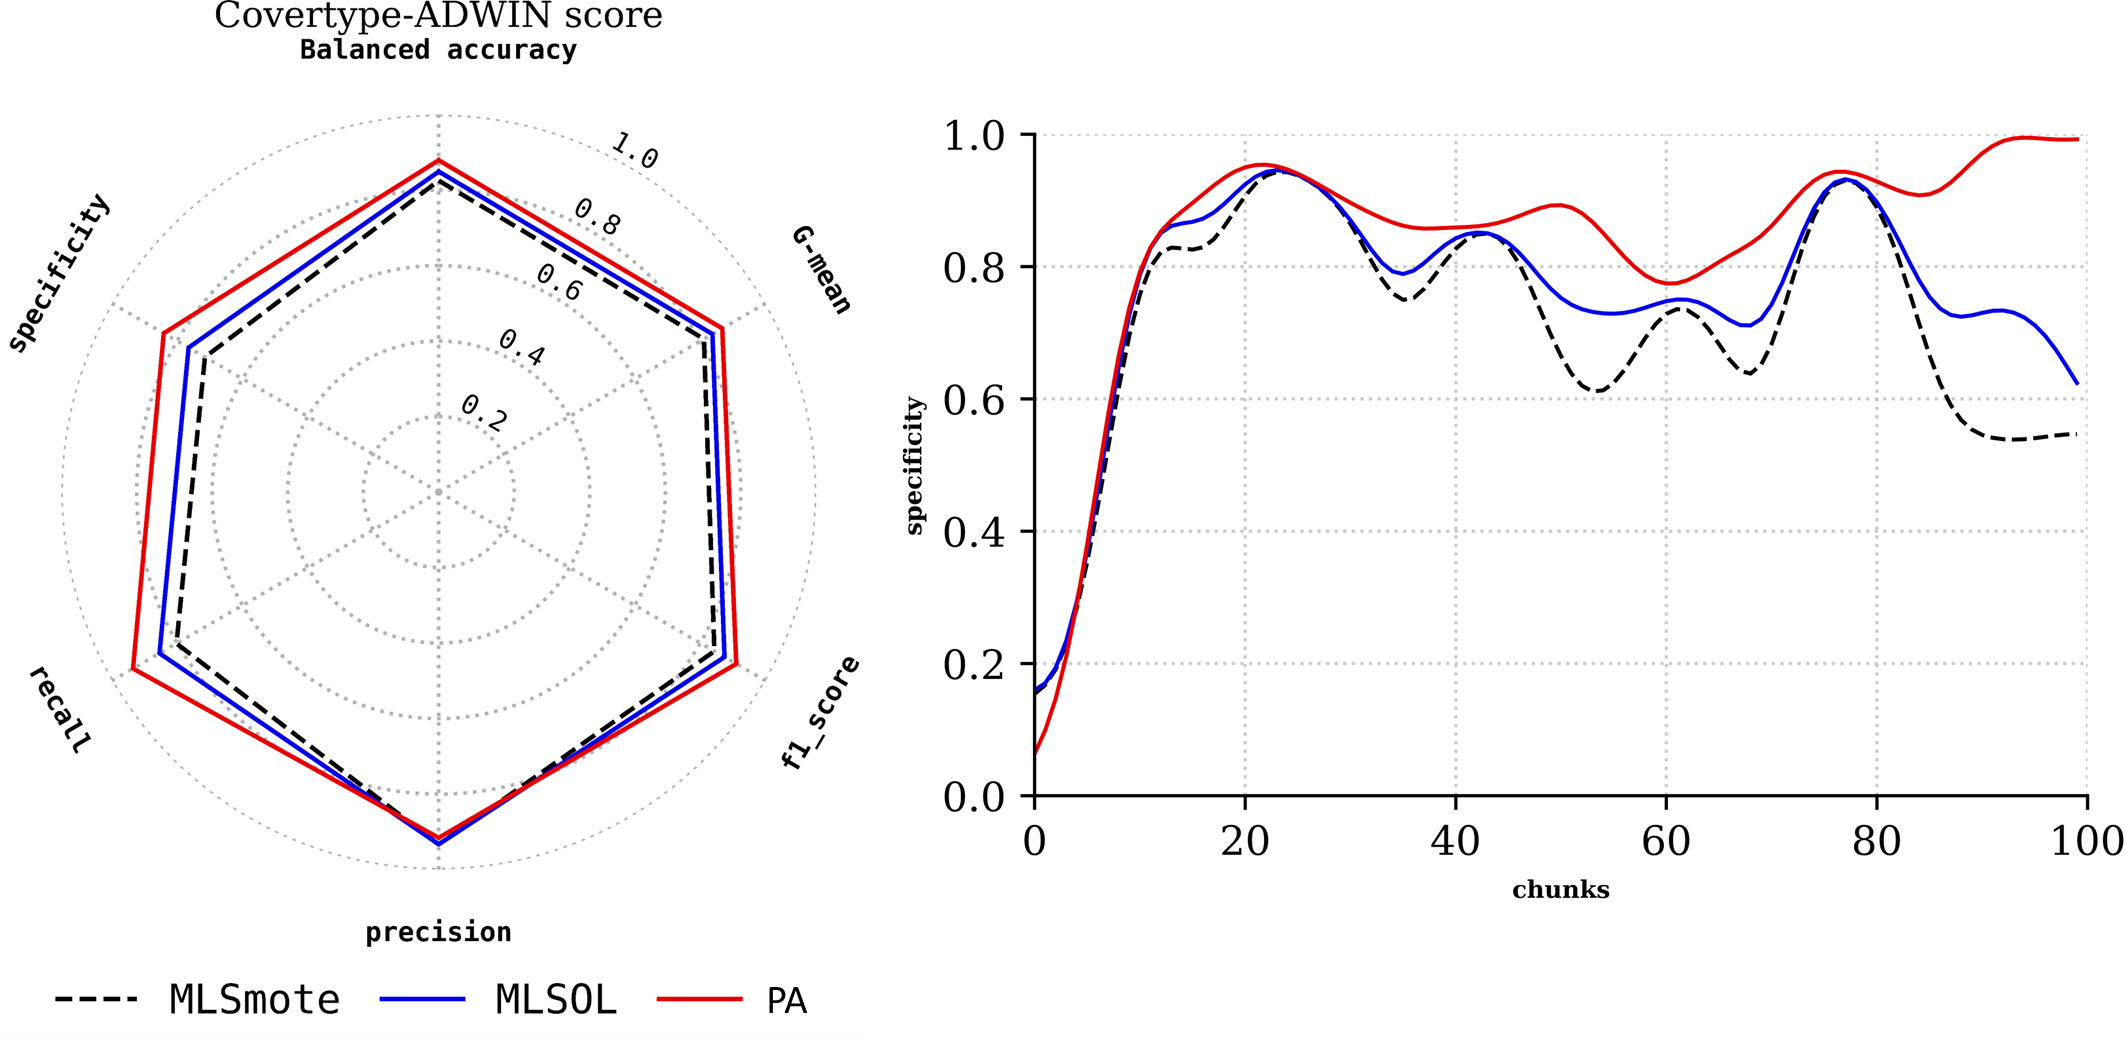
\includegraphics[width=1\linewidth]{4_Imbalanced/figures/exp_1.png}
	\caption{Synthetic Data Generator Flow.}
	\label{fig:4_first_proposal_result_exp_1}
\end{figure}

\begin{figure}[!ht]
	\centering
	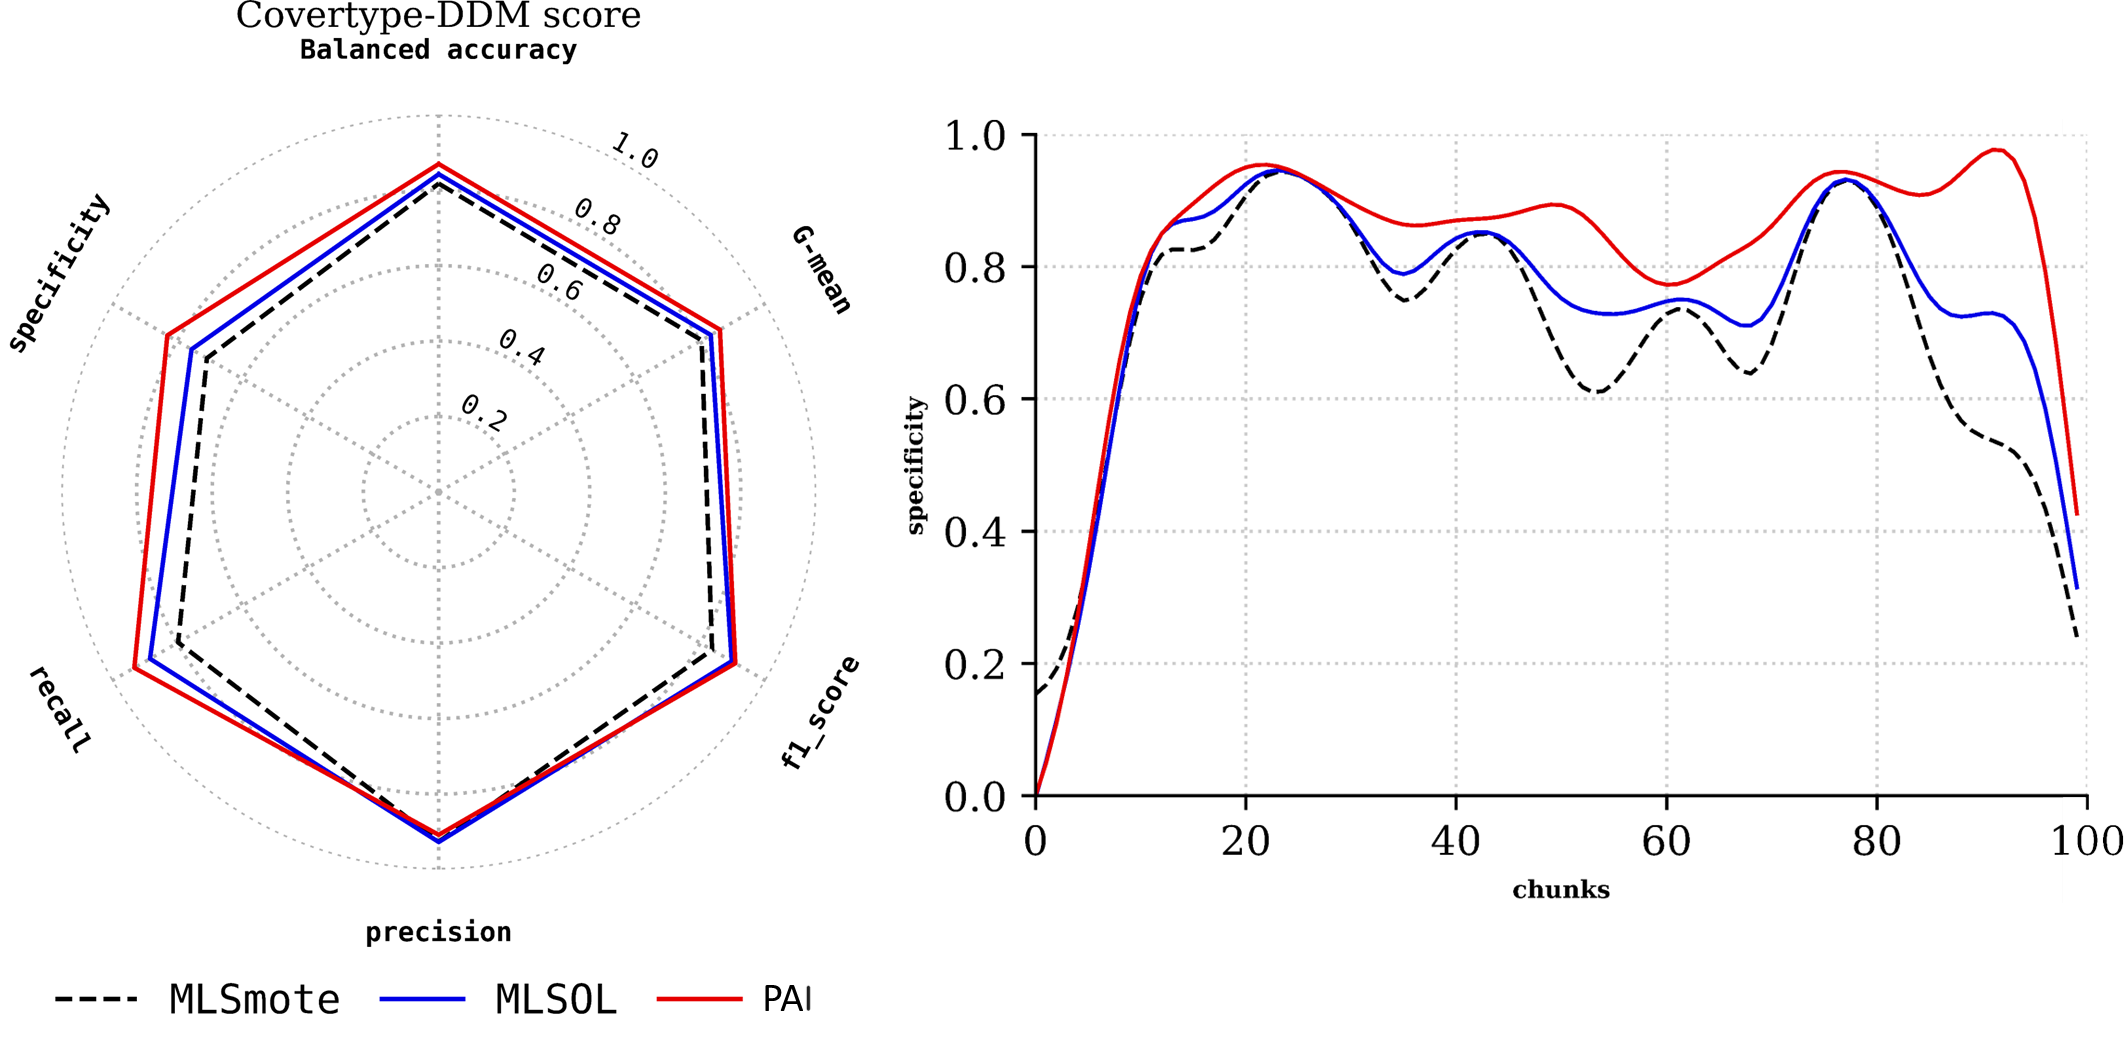
\includegraphics[width=1\linewidth]{4_Imbalanced/figures/exp_2.png}
	\caption{Synthetic Data Generator Flow.}
	\label{fig:4_first_proposal_result_exp_2}
\end{figure}

\subsubsection{Results on the Real Application Stream}
Fig. \ref{fig:4_first_proposal_result_exp_3} illustrates the outcomes of employing the three methods on the Sensor data stream using ADWIN as the drift detector. The radar graph depicts metric values ranging from 0.6 to 0.8, which indicate the pronounced drift and imbalance of the Sensor stream. In terms of the precision and recall metrics, the three methods exhibited almost identical values, whereas PA stood out in the other metrics. In contrast, MLSMOTE and MLSOL displayed similar values. By examining the line graph in Fig. \ref{fig:4_first_proposal_result_exp_3}
, it is evident that during the initial 30 chunks, PA's performance of PA might be suboptimal in some instances because of the limited number of classifiers in the pool. However, after the first 30 chunks, the performance significantly improved with the addition of more classifiers. In the same graph, PA consistently achieved the highest performance across all chunks, whereas MLSMOTE exhibited lower performance in certain chunks, and MLSOL exhibited lower performance in the other chunks. In Fig. \ref{fig:4_first_proposal_result_exp_4}, using the same dataset with the DDM as the drift detector, the radar plot metrics indicate lower results compared to the previous experiment. Nonetheless, the line graph underscores PA's dominance of PA in most chunks, although all methods exhibit nearly identical performance across the entire set of chunks. Overall, the performance of all the methods in Fig. \ref{fig:4_first_proposal_result_exp_4} is inferior to that in Fig. \ref{fig:4_first_proposal_result_exp_3} (ADWIN), which highlights ADWIN's superiority of ADWIN over DDM when applied to the Sensor data stream. 


\begin{figure}[!ht]
	\centering
	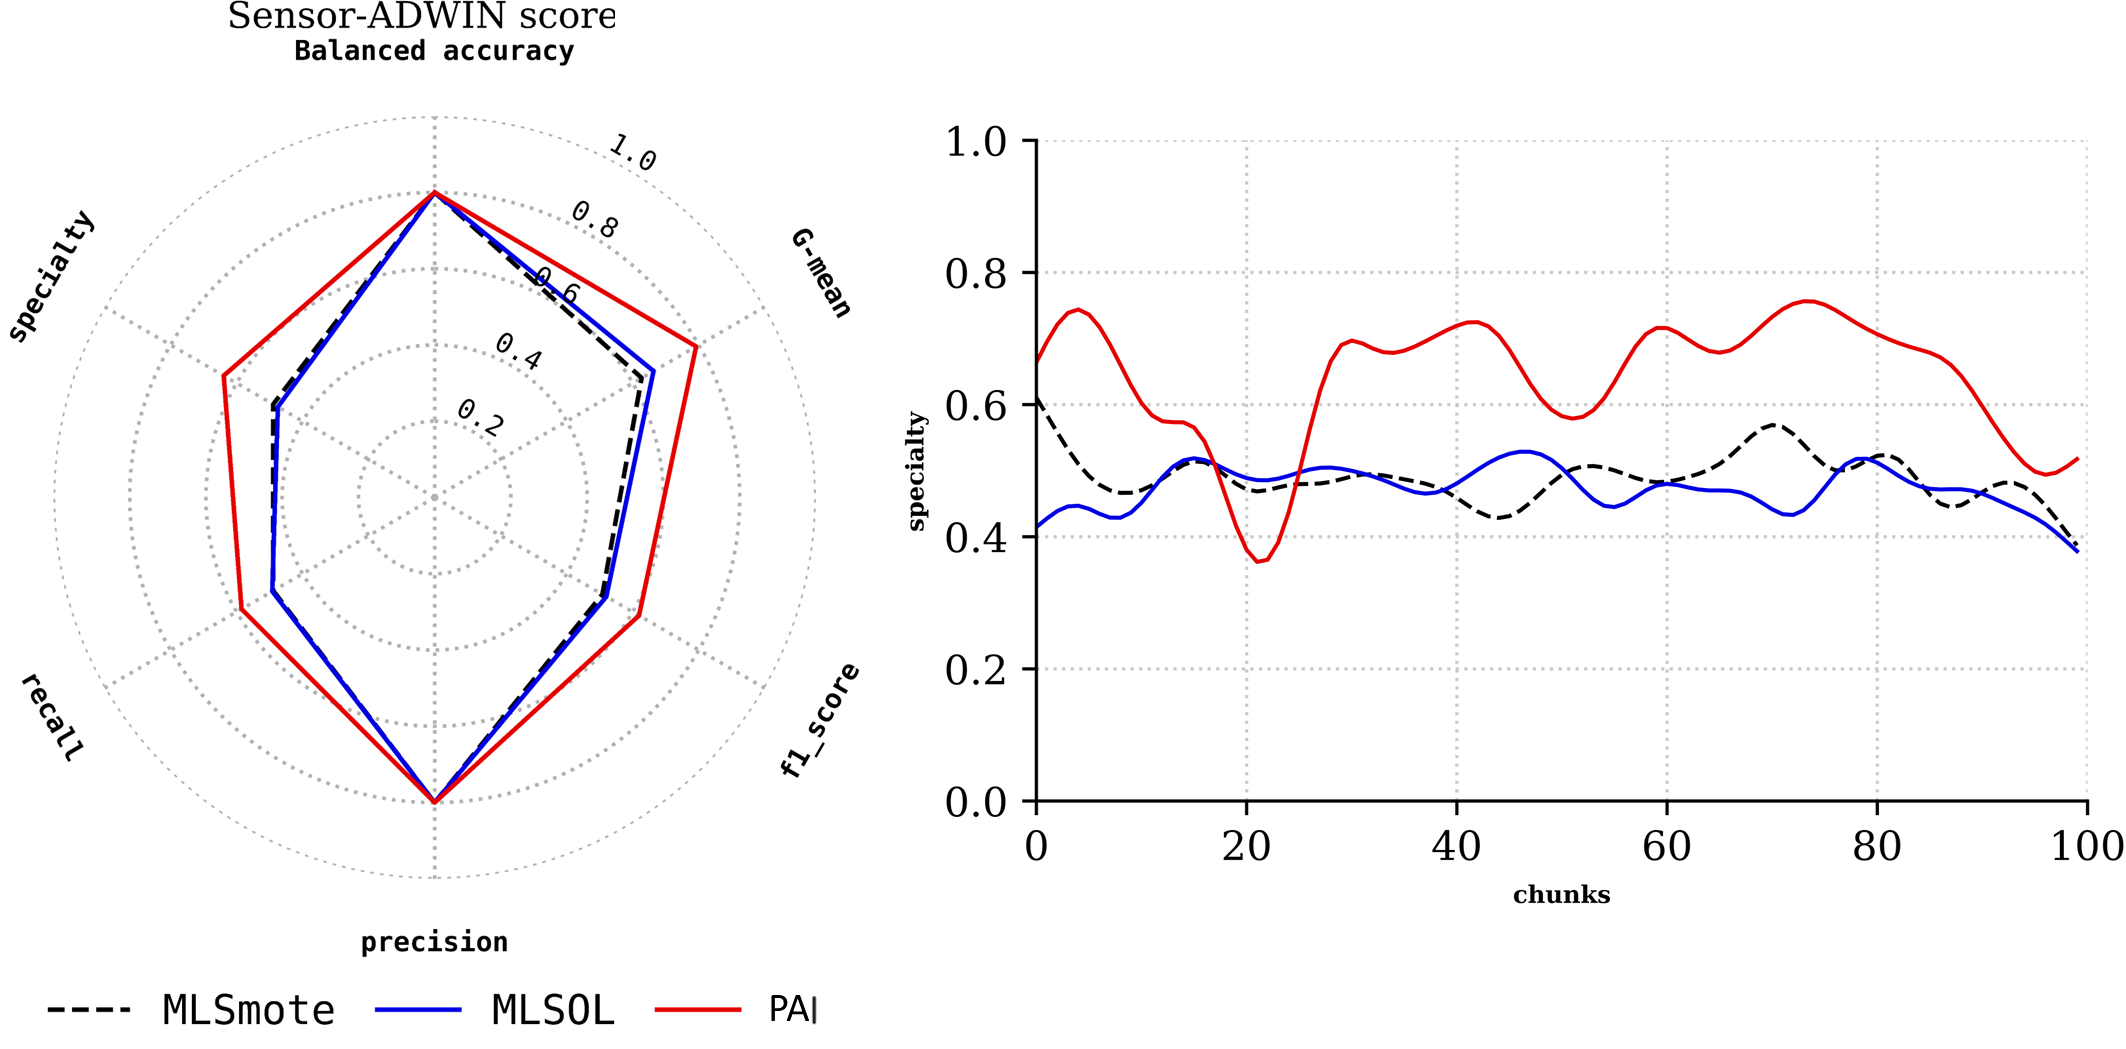
\includegraphics[width=1\linewidth]{4_Imbalanced/figures/exp_3.png}
	\caption{Synthetic Data Generator Flow.}
	\label{fig:4_first_proposal_result_exp_3}
\end{figure}

\begin{figure}[!ht]
	\centering
	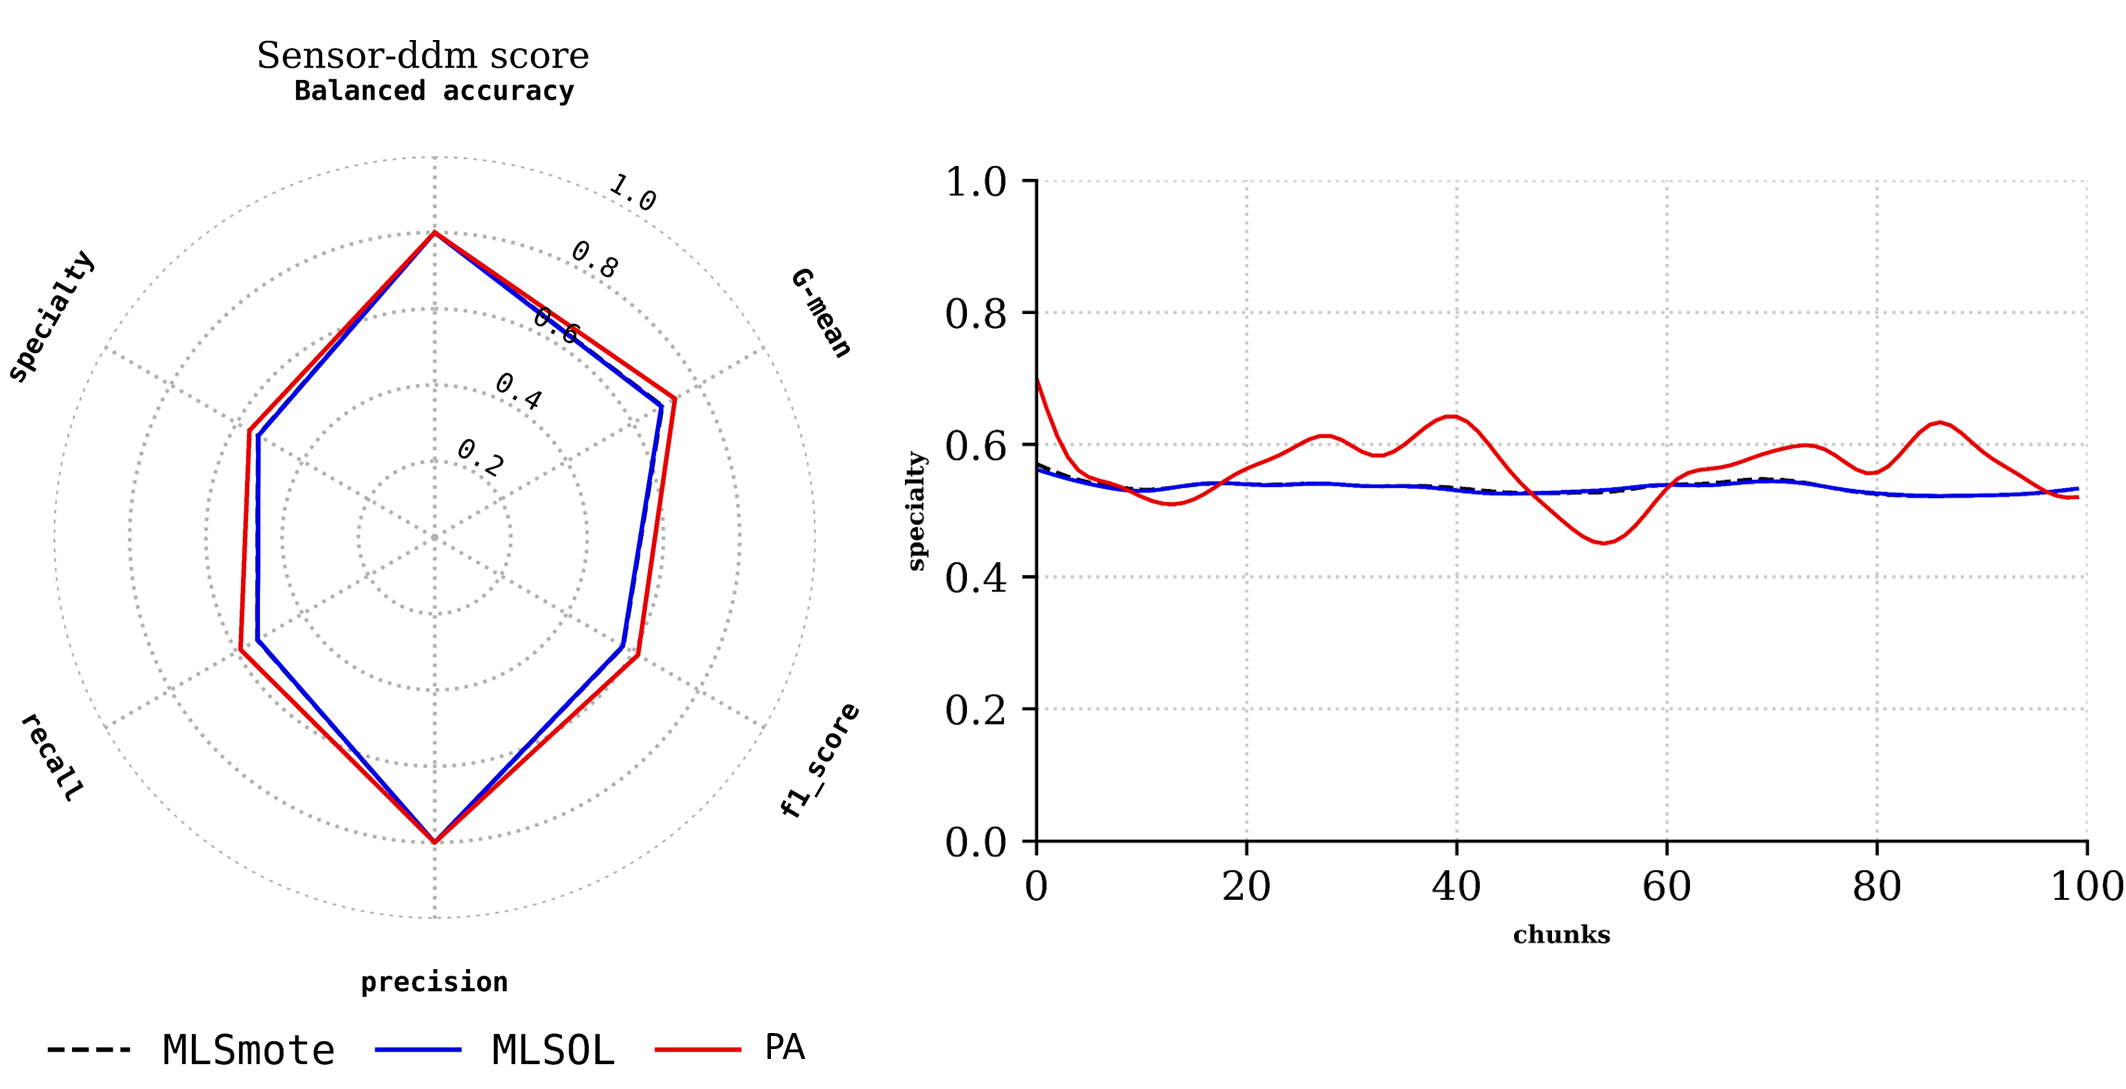
\includegraphics[width=1\linewidth]{4_Imbalanced/figures/exp_4.png}
	\caption{Synthetic Data Generator Flow.}
	\label{fig:4_first_proposal_result_exp_4}
\end{figure}


\subsubsection{Results on the Synthetic Stream}
The results of applying the same methods on the synthetic data stream using ADWIN as the drift detector are presented in Fig. \ref{fig:4_first_proposal_result_exp_5}. The radar diagram indicates metric values ranging from 0.6 to 0.8, suggesting that the synthetic stream is prone to frequent drifts. While MLSOL exhibited the highest precision, MLSOTE exhibited the lowest values. Conversely, PA performed well in other metrics, and MLSMOTE demonstrated the least favorable values. Upon examining the line diagram in Fig. \ref{fig:4_first_proposal_result_exp_5}, it becomes evident that during the initial ten chunks, the PA's performance might be suboptimal because of the limited number of classifiers in the pool. However, after the first ten chunks, the performance improved significantly with the inclusion of more classifiers. In the same diagram, PA consistently achieves the highest performance across all chunks, whereas MLSOL maintains satisfactory performance, and MLSMOTE exhibits lower performance throughout. In Fig. \ref{fig:4_first_proposal_result_exp_6}, using the same synthetic data stream but with the DDM as the drift detector, the radar plot metrics produce similar results to the previous experiment. However, the line diagram emphasizes the same outcomes as those in the previous experiment. Nevertheless, MLSOL and MLSMOTE achieved lower values than the previous experiment. These findings confirmed ADWIN's superiority of ADWIN over DDM when applied to synthetic data streams. These results highlight the versatility and robustness of the algorithm, demonstrating its effectiveness in handling concept drift across diverse datasets, including the challenging synthetic dataset, Covertype dataset, and Sensor dataset, regardless of whether ADWIN or DDM is used as the concept drift detector.

\begin{figure}[!ht]
	\centering
	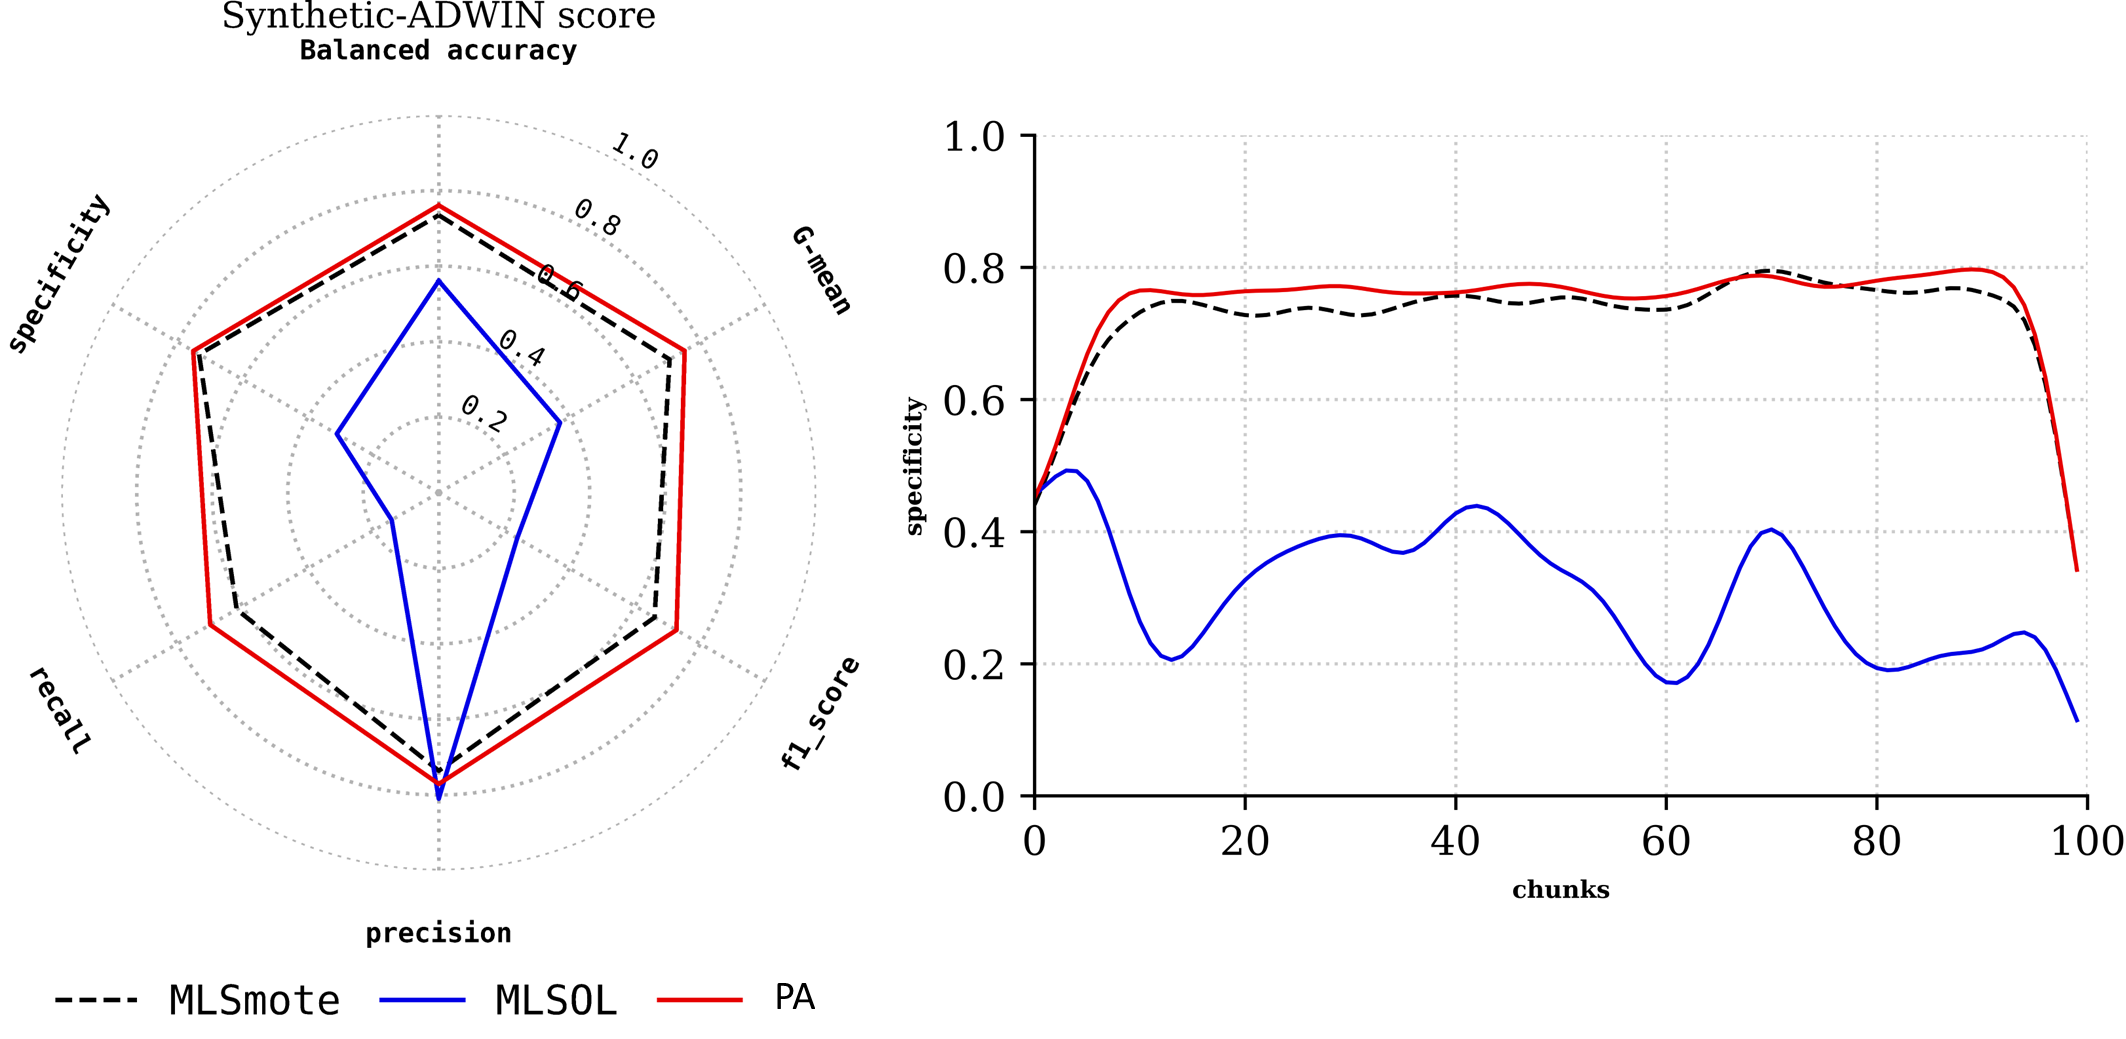
\includegraphics[width=1\linewidth]{4_Imbalanced/figures/exp_5.png}
	\caption{Synthetic Data Generator Flow.}
	\label{fig:4_first_proposal_result_exp_5}
\end{figure}

\begin{figure}[!ht]
	\centering
	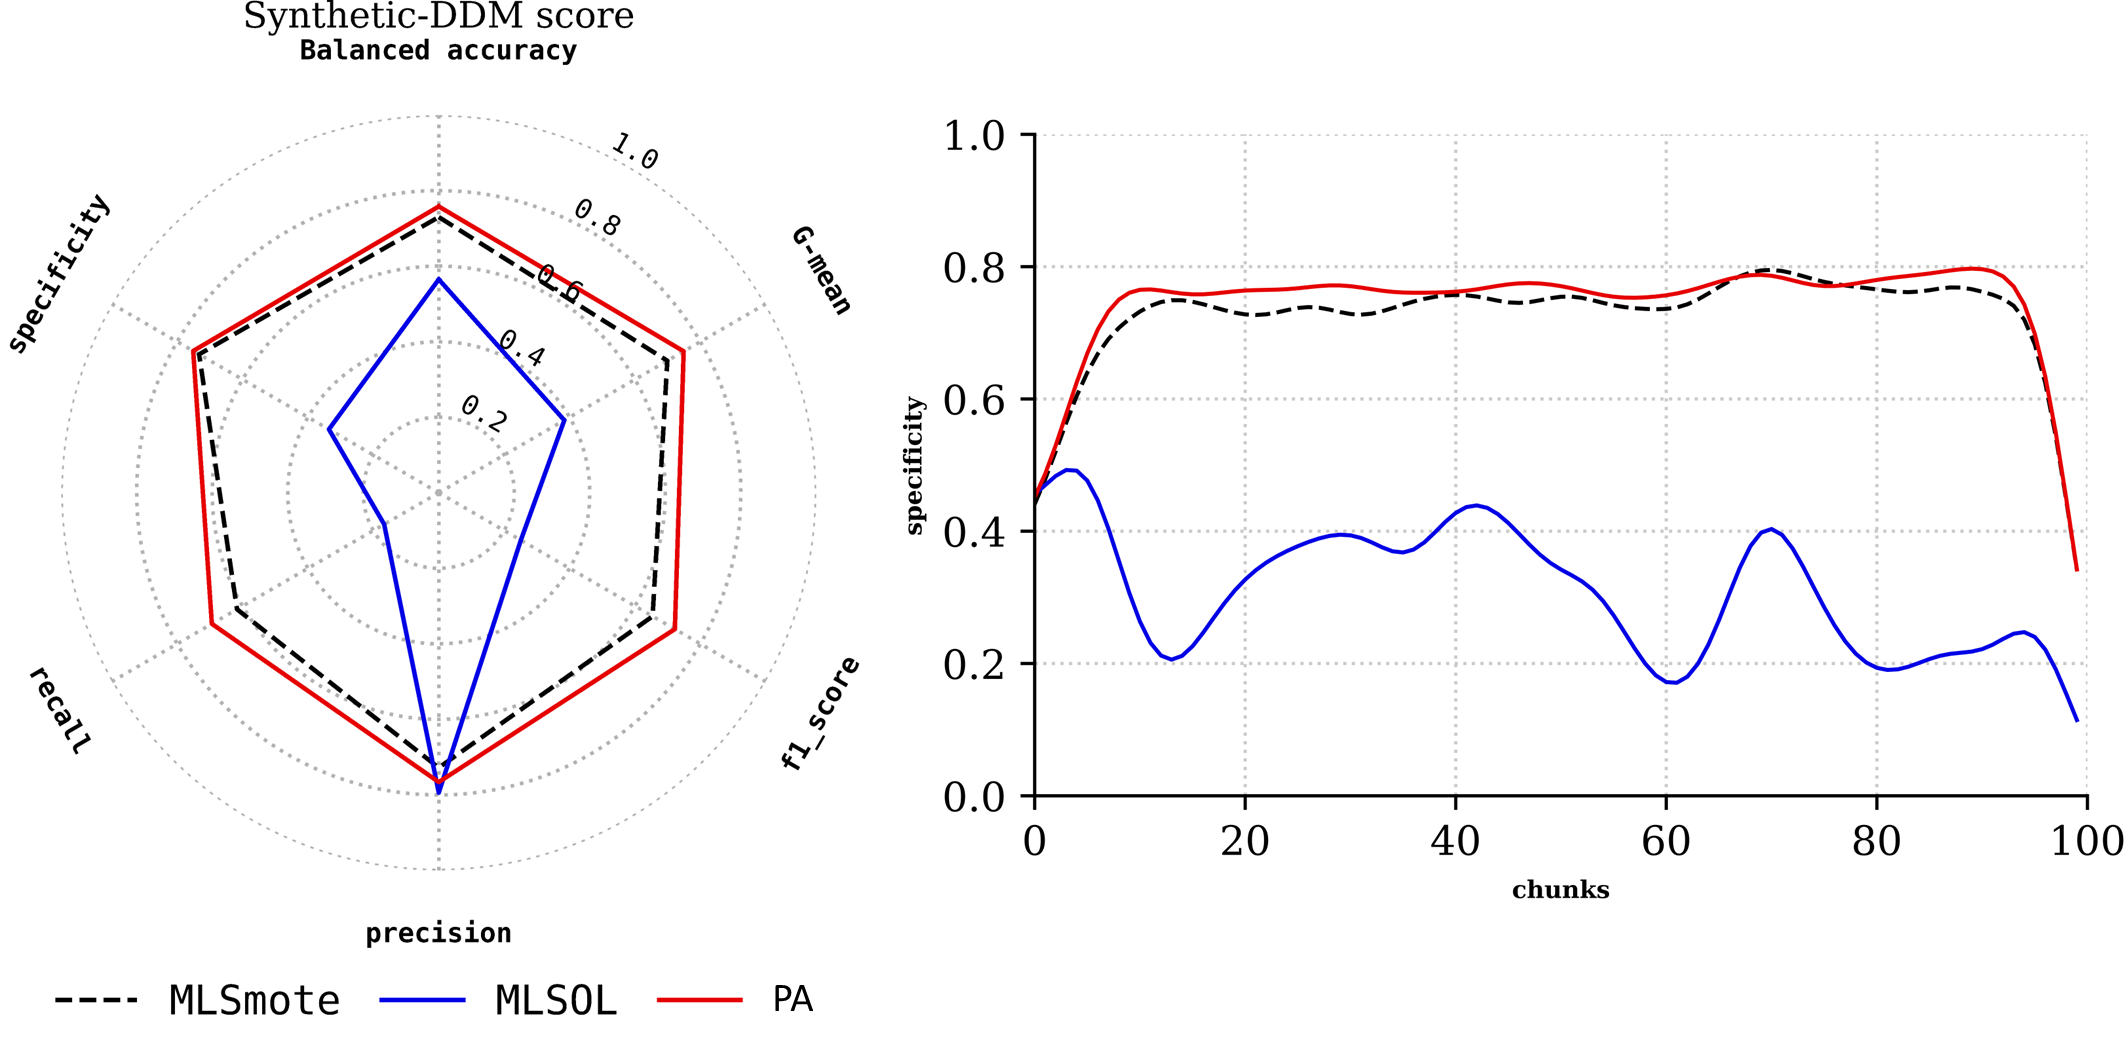
\includegraphics[width=1\linewidth]{4_Imbalanced/figures/exp_6.png}
	\caption{Synthetic Data Generator Flow.}
	\label{fig:4_first_proposal_result_exp_6}
\end{figure}


\subsection{Analysis of Class Overlap Factor between Proposed Approach (PA), MLSMOTE, and MLSOL Techniques.}
In our experimental study, we aimed to identify the critical factors that influence the selection of an optimal approach for minority classes in imbalanced drifted streams. These factors include various aspects, such as dataset characteristics, the choice of concept drift detectors, and the effectiveness of the algorithm in handling class overlap. To compare the overlapping class behavior of our proposed approach (PA) with MLSMOTE and MLSOL, we systematically designed experiments organized into groups of ten chunks. The results were visualized in bar diagrams, contrasting PA with other methods (MLSMOTE and MLSOL). Figures \ref{fig:4_first_proposal_result_exp_7}\ref{fig:4_first_proposal_result_exp_8}\ref{fig:4_first_proposal_result_exp_9} present ten groups, each with three bars representing MLSOTE, MLSOL, and PA, respectively. Each bar visually represents overlapped samples for ten chunks of several data streams, considering distinct concept drift detectors, specifically ADWIN and DDM.
Fig. \ref{fig:4_first_proposal_result_exp_7} shows two diagrams for the ADWIN and DDM detectors. In the ADWIN diagram, the third bar group (chunks 20-30) lacks overlapping samples because this chunk range does not have drifts, and no synthetic samples are generated for the training step. The sixth and tenth groups have the highest overlapped samples because these groups experience many drifts, leading to the generation of several samples and, consequently, the data indicates that MLSMOTE displays the highest number of overlapping samples across all groups, while PA exhibits very few, except for the last group (90-100), which has a small number of overlapping samples. However, the DDM diagram has more overlapping samples than the ADWIN diagram because the DDM detector detects fewer drifts than ADWIN. Specifically, the last value on the Y-axis of the ADWIN diagram is 3,000 samples, while the last value on the Y-axis of the DDM diagram is 2,000 samples. Fig. \ref{fig:4_first_proposal_result_exp_8} and Fig. \ref{fig:4_first_proposal_result_exp_9} display the overlapping samples of the three methods on the Sensor and synthetic data streams, respectively. In Fig. \ref{fig:4_first_proposal_result_exp_8}, the ADWIN diagram demonstrates fewer overlapped samples than in Fig. \ref{fig:4_first_proposal_result_exp_8}, indicating a lower number of drifts in the Sensor stream. The overall diagram indicates that our proposed approach achieves fewer overlapped samples than MLSOL and MLSMOTE, with MLSMOTE having the highest number of overlapped samples. In the DDM diagram of Fig. 10, the number of overlapped samples is lower than in Fig. \ref{fig:4_first_proposal_result_exp_7}, with our proposed approach consistently achieving the lowest number of overlapped samples across most group bars.
In Fig. \ref{fig:4_first_proposal_result_exp_9}, the ADWIN and DDM diagrams exhibit the greatest number of overlapped samples compared to the earlier figures. This suggests that the synthetic stream underwent frequent drifts and was more susceptible to noise. Consequently, the last value on the Y-axis in both the ADWIN and DDM diagrams was recorded for 7,000 samples. Our proposed approach consistently achieves the lowest number of overlapped samples, whereas MLSMOTE consistently attains the highest number of overlapped samples across most group bars in both the ADWIN and DDM diagrams. In conclusion, our thorough examination of overlapping class instances across MLSMOTE, MLSOL, and our proposed approach consistently reveals minimal overlapped samples compared to other methods, regardless of whether DDM or ADWIN is employed as drift detectors

\begin{figure}[!ht]
	\centering
	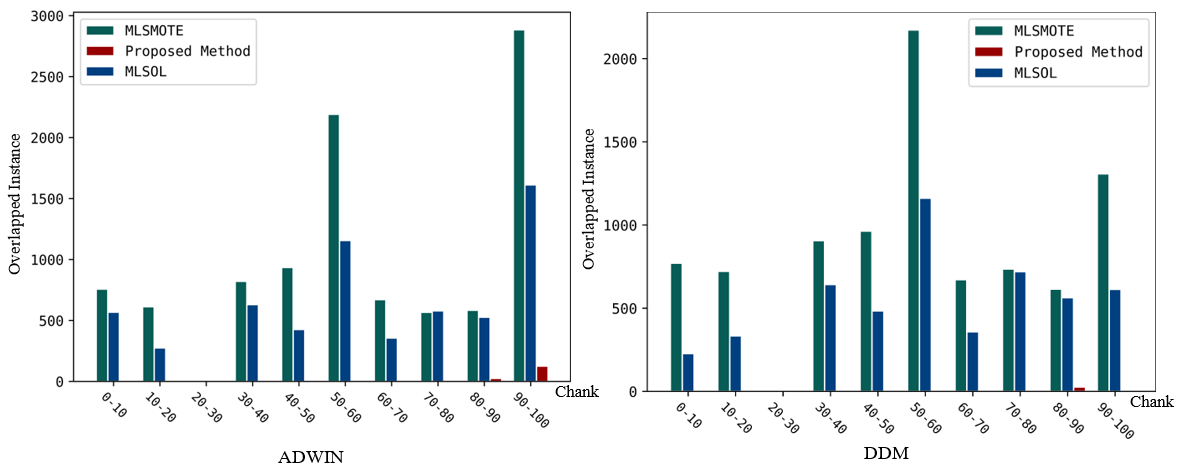
\includegraphics[width=1\linewidth]{4_Imbalanced/figures/exp_7.png}
	\caption{Synthetic Data Generator Flow.}
	\label{fig:4_first_proposal_result_exp_7}
\end{figure}

\begin{figure}[!ht]
	\centering
	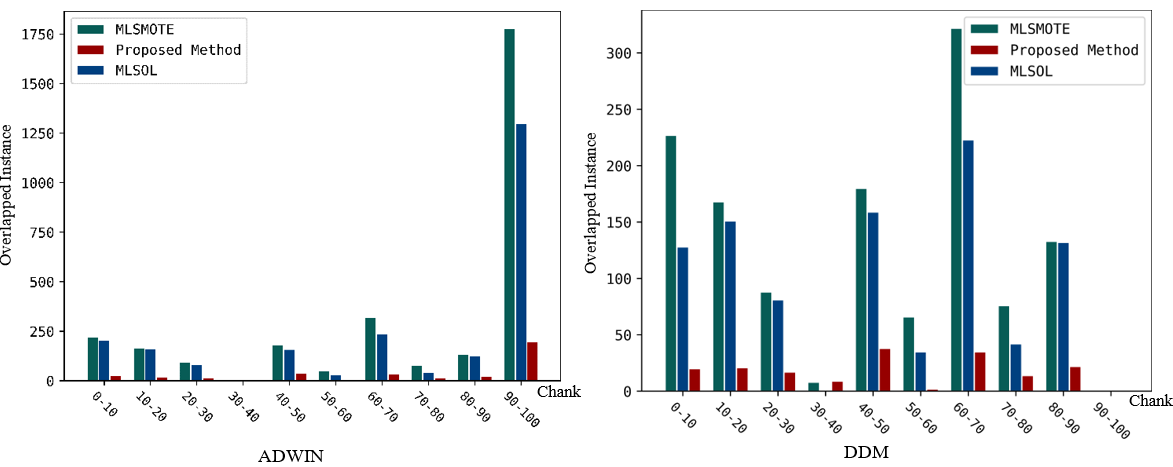
\includegraphics[width=1\linewidth]{4_Imbalanced/figures/exp_8.png}
	\caption{Synthetic Data Generator Flow.}
	\label{fig:4_first_proposal_result_exp_8}
\end{figure}

\begin{figure}[!ht]
	\centering
	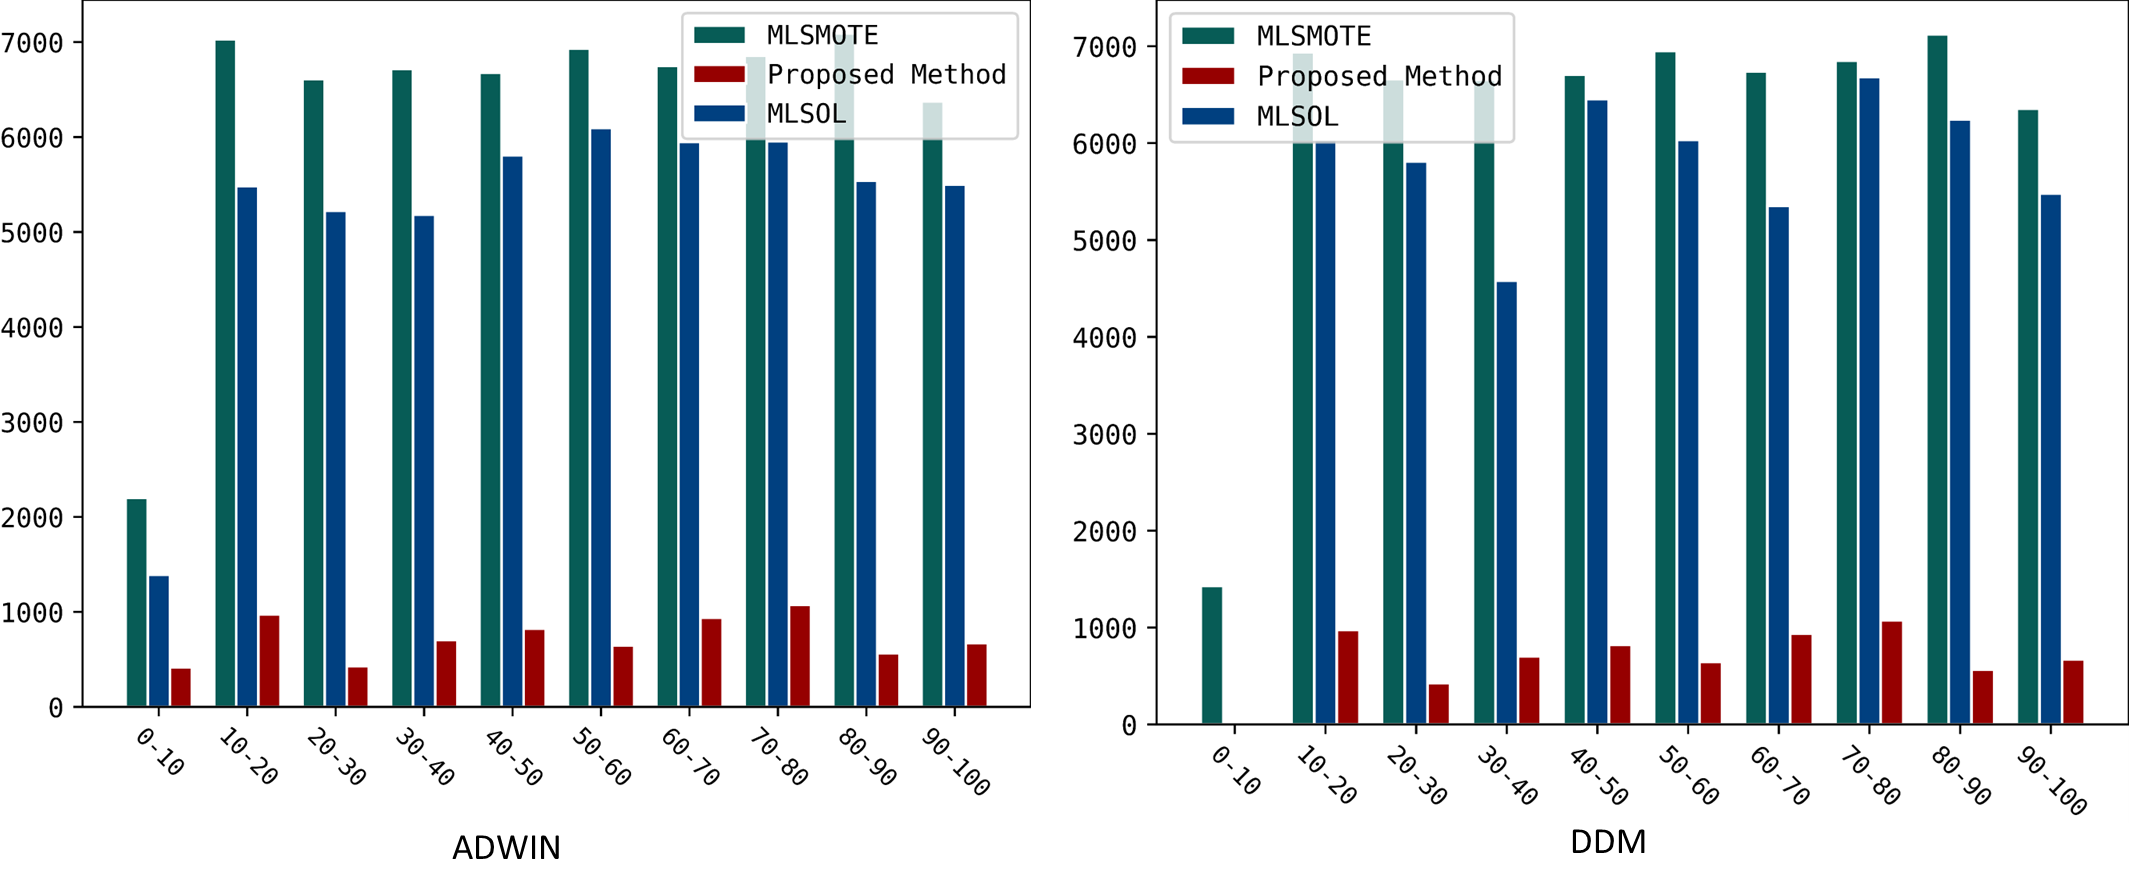
\includegraphics[width=1\linewidth]{4_Imbalanced/figures/exp_9.png}
	\caption{Synthetic Data Generator Flow.}
	\label{fig:4_first_proposal_result_exp_9}
\end{figure}

\subsection{Analyzing Runtime Factor Between the Proposed Approach, MLSMOTE, and MLSOL Techniques}
The results of our experiments indicate that the choice of the best algorithm for multiclass imbalanced streams depends on various factors, including dataset characteristics, the concept drift detector used, the presence of an overlapping class problem, and the algorithm's runtime demands. To investigate the runtimes of MLSMOTE, MLSOL, and our proposed approach, we conducted experiments, as shown in Table \ref{tab:4_first_proposal_result_table_2}. Our findings reveal that our proposed approach is highly efficient, regardless of whether ADWIN or DDM is used as the concept drift detector. Specifically, when ADWIN was used, the proposed approach algorithm took 8344 s to train and predict the Covertype stream for ensemble classifiers, whereas it took 8019 s when using the DDM detector. In contrast, MLSMOTE and MLSOL require more time for the same task. Notably, our proposed approach maintains efficiency, even when using the DDM concept detector. Additionally, our proposed approach demonstrates shorter processing times in the Sensor stream and synthetic data compared with other methods. Consistently, the DDM detector achieved less time across all experiments owing to its lower detection of drifts compared to the ADWIN detector. This is because there are fewer instances that trigger training for pool classifiers when using the DDM. The bold highlighting in Table \ref{tab:4_first_proposal_result_table_2} further emphasizes the efficiency of our proposed approach with both the ADWIN and DDM detectors across all dataset streams. Because our proposal generates fewer overlapped samples, leading to an overall decrease in the running time.

\begin{table}[h!]
  \centering
  \resizebox{\textwidth}{!}{
  \begin{tabular}{|l|l|c|c|c|}
  \hline
  \textbf{Stream} & \textbf{Concept Drift Detector} & \textbf{MLSMSOTE} & \textbf{MLSOL} & \textbf{PA} \\ \hline
  \multirow{2}{*}{Benchmark} & ADWIN & 9559 & 8655 & \textbf{8344} \\ \cline{2-5} 
   & DDM & 8388 & 8031 & \textbf{8019} \\ \hline
  \multirow{2}{*}{Real Application} & ADWIN & 1291 & 1310 & \textbf{1102} \\ \cline{2-5} 
   & DDM & 585 & 607 & \textbf{521} \\ \hline
  \multirow{2}{*}{Synthetic} & ADWIN & 12870 & 4866 & \textbf{4834} \\ \cline{2-5} 
   & DDM & 12397 & 4958 & \textbf{4687} \\ \hline
  \end{tabular}
  }
  \caption{Runtime of MLSMOTE, MLSOLE, and Proposed Approach (PA)}
  \label{tab:4_first_proposal_result_table_2}
  \end{table}

\subsection{Analyzing Non-parametric Tests between the Proposed Approach, MLSMOTE, and MLSOL Techniques}
We conducted a thorough series of statistical analyses encompassing 12 comparisons across three diverse datasets, three methods, and two drift detectors. These analyses were rigorously evaluated using a non-parametric test, specifically the Kruskal-Wallis test. The results of this test were striking, revealing substantial variations in the G-mean measurements across most experiments. Importantly, these differences were not due to random chance \cite{yamada2013change}. Upon closer examination of the assessments for the three methods, PA, MLSMOTE, and MLSOTE, as detailed in Table \ref{tab:4_first_proposal_result_table_3}, we found compelling evidence supporting the acceptance of the null hypothesis (H0).
This implies that the expected and observed data exhibited statistically significant disparities. H0 is rejected when significant differences are not observed and H0 is accepted if the P-value falls below the critical value. Underlining the significance of our analysis, the Kruskal-Wallis test was conducted with a 95\% confidence level, and the P-value was rounded to the first three digits after the decimal point. Nevertheless, it is important to note that a similarity in the performances of the methods emerged in the third and fourth experiments, resulting in the rejection of H0. This similarity can be attributed to the fact that the DDM detected fewer drifts in these experiments.


\begin{table}[h!]
  \centering
  \resizebox{\textwidth}{!}{
  \begin{tabular}{|c|c|c|c|c|c|}
  \hline
  \multirow{2}{*}{Dataset} & \multirow{2}{*}{Drift detector} & \multirow{2}{*}{Comparison} & \multirow{2}{*}{P-value} & \multirow{2}{*}{Critical value} & \multirow{2}{*}{H0} \\ 
                           &                                 &                             &                           &                                 &  \\
  \hline
  \multirow{4}{*}{Covertype stream} & \multirow{2}{*}{ADWIN} & PA - MLSSMOTE & 0.001 & 0.05 & Accept \\ \cline{3-6}
                                    &                        & PA - MLSOL    & 0.014 & 0.05 & Accept \\ \cline{2-6}
                                    & \multirow{2}{*}{DDM}   & PA - MLSSMOTE & 0.361 & 0.05 & Rejected \\ \cline{3-6}
                                    &                        & PA - MLSOL    & 0.401 & 0.05 & Rejected \\ 
  \hline
  \multirow{4}{*}{Sensor stream} & \multirow{2}{*}{ADWIN} & PA - MLSSMOTE & 0.001 & 0.05 & Accept \\ \cline{3-6}
                                 &                        & PA - MLSOL    & 0.001 & 0.05 & Accept \\ \cline{2-6}
                                 & \multirow{2}{*}{DDM}   & PA - MLSSMOTE & 0.001 & 0.05 & Accept \\ \cline{3-6}
                                 &                        & PA - MLSOL    & 0.001 & 0.05 & Accept \\ 
  \hline
  \multirow{4}{*}{Synthetic stream} & \multirow{2}{*}{ADWIN} & PA - MLSSMOTE & 0.001 & 0.05 & Accept \\ \cline{3-6}
                                    &                        & PA - MLSOL    & 0.001 & 0.05 & Accept \\ \cline{2-6}
                                    & \multirow{2}{*}{DDM}   & PA - MLSSMOTE & 0.001 & 0.05 & Accept \\ \cline{3-6}
                                    &                        & PA - MLSOL    & 0.001 & 0.05 & Accept \\ 
  \hline
  \end{tabular}
  }
  \caption{Kruskal-Wallis test between MLSMOTE, MLSOLE, and Proposed Approach (PA)}
  \label{tab:4_first_proposal_result_table_3}
  \end{table}